Let 
%
\begin{align}
    \Vec{A}=\myvec{1\\-2},
    \Vec{B}=\myvec{-3\\4}
\end{align}
%
Then, 
\begin{align}
\vec{Q}&=\frac{2\myvec{-3\\4}+1\myvec{1\\-2}}{\brak{1+2}}   \\
&
=\myvec{\frac{-5}{3}\\[0.2cm]{2}}
\\
\vec{P}&=\frac{1\myvec{-5/3\\2}+1\myvec{1\\-2}}{\brak{1+1}}   
\\
&=\myvec{\frac{-1}{3} \\[0.2cm]{0}}
\end{align}
Fig. \ref{1/19/python fig1.png} verifies the result.
\begin{figure}[!ht]
\centering
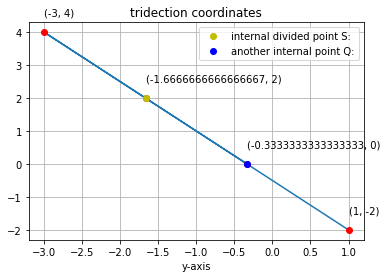
\includegraphics[width=\columnwidth]{solutions/1/19/assignment.1.pythom plot.png}
\caption{ Plot of coordinates}
\label{1/19/python fig1.png}
\end{figure}


